\documentclass[
	9pt,
	hyperref = {unicode,pdfpagelabels=false},
	notheorems,
	aspectratio=169
	]{beamer}
\mode<presentation>

\usetheme{metropolis}
\metroset{
	progressbar = foot,
	block = fill,
}

\usefonttheme{professionalfonts}
\setsansfont{IBM Plex Sans}
\setmonofont{IBM Plex Mono}

\usepackage[english]{babel}
\usepackage{
		amsmath,
		tikz,
		mathtools,
		tikz-3dplot,
		calc,
		enumitem,
		subcaption,
		booktabs,
}

\mathtoolsset{showonlyrefs,showmanualtags}


\let\d\undefined
\let\div\undefined
\newcommand{\d}{\partial}
\DeclareMathOperator{\div}{div}
\DeclareMathOperator{\grad}{grad}


\title{codename: OptiPuls}
\subtitle{an optimal control problem for\\single spot pulsed laser welding}
\titlegraphic{\vspace{0.6cm}\flushright\includegraphics[height=3cm]{plots/static/logo.pdf}}
\author{Dmytro Strelnikov, Roland Herzog}
\institute{Technische Universität Chemnitz \\ Technische Universität Ilmenau}
\date{Bayreuth 2021}


\begin{document}
\maketitle

\begin{frame}{Single spot pulsed laser welding and hot cracks}
\begin{figure}
		\centering
	\begin{subfigure}[b]{.5\textwidth}
		\centering
		% !TEX root = ../talk.tex

\newcommand{\varR}{2.5}
\newcommand{\varr}{1}
\newcommand{\vardi}{0.5}
\newcommand{\vardii}{0.8}
\newcommand{\varrlas}{0.4}
\newcommand{\varhlas}{0.5}

\definecolor{mycoral}{RGB}{236,27,75}
\definecolor{myorange}{RGB}{242,106,68}

\begin{tikzpicture}[scale=1.2]

	% fillers
	\draw [draw=none, fill=gray!35] (-\varR,0) rectangle (\varR,-\vardi);
	\draw [draw=none, fill=gray!15] (-\varR,-\vardi) rectangle (\varR,-\vardi-\vardii);

	% lines
	\draw (-\varR,-\vardi) -- (\varR,-\vardi);
	\draw (-\varR,-\vardi-\vardii) -- (\varR,-\vardi-\vardii);
	\draw (-\varR,0) -- (-\varr,0);
	\draw (\varr,0) -- (\varR,0);

	\draw [myorange, thick, fill=myorange!25] (0,0) ++(180:\varr) arc (180:360:\varr);

	% laser
	\draw [->, ultra thick, color=mycoral] (0,\varhlas) -- (0,0);

	% captions
	\draw (0,.5*\varhlas) node [left] {\small laser beam};
	\draw (1.2*\varr,-.5*\vardi) node [right] {\small sheet A};
	\draw (1.2*\varr,-\vardi-.5*\vardii) node [right] {\small sheet B};
	\draw (0,-.5*\varr) node {\small liquid melt};
\end{tikzpicture}

	\end{subfigure}%
	\begin{subfigure}[b]{.5\textwidth}
		\centering
		%!TeX root = ../tui19-talk-ws.tex

\newcommand{\varR}{2.5}
\newcommand{\varr}{1}
\newcommand{\vardi}{0.5}
\newcommand{\vardii}{0.8}
\newcommand{\varrlas}{0.4}
\newcommand{\varhlas}{0.8}

\definecolor{mycoral}{RGB}{236,27,75}
\definecolor{myorange}{RGB}{242,106,68}

\begin{tikzpicture}[scale=1.2]



	% fillers
	\draw [draw=none, fill=gray!35] (-\varR,0) rectangle (\varR,-\vardi);
	\draw [draw=none, fill=gray!15] (-\varR,-\vardi) rectangle (\varR,-\vardi-\vardii);



	% lines
	\draw (-\varR,-\vardi) -- (\varR,-\vardi);
	\draw (-\varR,-\vardi-\vardii) -- (\varR,-\vardi-\vardii);
	% \draw (-\varR,0) -- (-\varr,0);
	% \draw (\varr,0) -- (\varR,0);


	\draw [very thin, fill=gray!25] (0,0) ++(180:\varr) arc (180:360:\varr);

	% Crack
	\draw [thick] (1.9-2, -0.8) -- (1.99-2, -0.7) -- (1.872-2, -0.5) -- (1.92-2, -0.35) -- (1.88-2, -0.25) -- (1.93-2, -0.18)  -- (1.87-2, -0.12) -- (1.92-2, -0.04) -- (1.96-2, -0.05) -- (0,0);
	\draw [thick] (1.6-2,-0.7) -- (1.65-2, -0.6) -- (1.78-2, -0.61) -- (1.872-2, -0.5);
	\draw [thick] (2.05-2, -0.95) -- (2.1-2, -0.8) -- (1.99-2,-0.7);
	\draw [thick] (2.2-2, -0.85) -- (2.1-2, -0.8);

	\draw (-\varR,0) -- (\varR,0);
\end{tikzpicture}

	\end{subfigure}
	\caption{Illustration of a single spot laser welding and undesired hot crack after solidification.}
	\label{fig:welding}
	\end{figure}

	According to our current understanding of the problem, the hot cracks appear because the solidification front moves too fast during the cooling stage.
	Hence, we aim at reduction of the solidification speed by controlling the laser power profile in time.

	\begin{figure}
		\centering
		% !TEX root = ../talk.tex

\newcommand{\varR}{2.5}
\newcommand{\varr}{1}
\newcommand{\vardi}{0.5}
\newcommand{\vardii}{0.8}
\newcommand{\varrlas}{0.4}
\newcommand{\varhlas}{0.8}

\definecolor{mycoral}{RGB}{236,27,75}
\definecolor{myorange}{RGB}{242,106,68}

\begin{tikzpicture}[scale=1.2]

	% fillers
	\draw [draw=none, fill=gray!35] (-\varR,0) rectangle (\varR,-\vardi);
	\draw [draw=none, fill=gray!15] (-\varR,-\vardi) rectangle (\varR,-\vardi-\vardii);

	% lines
	\draw (-\varR,-\vardi) -- (\varR,-\vardi);
	\draw (-\varR,-\vardi-\vardii) -- (\varR,-\vardi-\vardii);
	\draw (-\varR,0) -- (-\varr,0);
	\draw (\varr,0) -- (\varR,0);

	\draw [myorange, thick, fill=myorange!25] (0,0) ++(180:\varr) arc (180:360:\varr);

	% velocity
	% \foreach \angle in {-180, -135, -90, -45, 0}
	\foreach \angle in {-180, -150, -120, -90, -60, -30, 0}
	{
		\draw [->, myorange, thick] ({\varr*cos(\angle)}, {\varr*sin(\angle)}) -- ({0.75*\varr*cos(\angle)}, {0.75*\varr*sin(\angle)});
	}

\end{tikzpicture}

		\caption{Solidification interface and its velocity.}
	\end{figure}
\end{frame}


\begin{frame}{Modelling challenges: enthalpy of fusion and convective heat transfer}
	\begin{minipage}{0.5\textwidth}
		The enthalpy of fusion and the convective heat transfer in the liquid phase become the modelling challenges caused by the phase transition.\\
		We include them in the model by adjusting the coefficients of the heat equation.
	\end{minipage}%
	\begin{minipage}{0.5\textwidth}
		\begin{figure}
			\centering
			% !TEX root = ../talk.tex

\newcommand{\varR}{2.5}
\newcommand{\varr}{1}
\newcommand{\vardi}{0.5}
\newcommand{\vardii}{0.8}
\newcommand{\varrlas}{0.4}
\newcommand{\varhlas}{0.4}

\definecolor{mycoral}{RGB}{236,27,75}
\definecolor{myorange}{RGB}{242,106,68}

\begin{tikzpicture}[scale=1.2]

	% fillers
	\draw [draw=none, fill=gray!35] (-\varR,0) rectangle (\varR,-\vardi);
	\draw [draw=none, fill=gray!15] (-\varR,-\vardi) rectangle (\varR,-\vardi-\vardii);

	% lines
	\draw (-\varR,-\vardi) -- (\varR,-\vardi);
	\draw (-\varR,-\vardi-\vardii) -- (\varR,-\vardi-\vardii);
	\draw (-\varR,0) -- (-\varr,0);
	\draw (\varr,0) -- (\varR,0);

	\draw [myorange, thick, fill=myorange!25] (0,0) ++(180:\varr) arc (180:360:\varr);

	% laser
	\draw [->, ultra thick, color=mycoral] (0,\varhlas) -- (0,0);

	% convection
	\draw[>->, thick, color=myorange, yscale=1.0] (-0.1, -0.4) arc (0:290:0.35);
	\draw[>->, thick, color=myorange, yscale=1.0] (0.1, -0.4) arc (180:-110:0.35);

	% heat transition
	\draw [->, thick, color=mycoral] (0.2, 0.1) -- (1, 0.1) node [midway, above] {\small heat};
	\draw [->, thick, color=mycoral] (-0.2, 0.1) -- (-1, 0.1) node [midway, above] {\small heat};
	\draw [->, thick, color=mycoral] (0, -0.9) -- (0, -0.5);

\end{tikzpicture}

			\caption{Convective flows due to the Marangoni effect.}
			\label{fig:convection}
		\end{figure}
	\end{minipage}
	\vspace{-1.5em}
	\begin{figure}
		\centering
		\includegraphics{plots/coefficients/vhc.pdf}%
		\includegraphics{plots/coefficients/kappa.pdf}
		\vspace{-1.2em}
		\caption{Effective volumetric heat capacity $s(\theta)$ and effective thermal conductivity $\kappa(\theta)$\\ constructed using spline fitting procedure.}
		\label{fig:heat_capacity}
	\end{figure}
\end{frame}


\begin{frame}{Domain geometry}
Let $\Omega	\subset \mathbb{R}^3$ be an open right circular cylinder and $\Gamma = \cup_{i=1}^4 \Gamma_i$ be its surface.

	\begin{figure}
		%!TeX root = ../numapde-OptiPuls-2.tex

\newcommand{\varR}{3.0}
\newcommand{\varr}{1.0}
\newcommand{\varZ}{2.5}

% top view (xy)
% \tdplotsetmaincoords{0}{0}
% side view (xz)
% \tdplotsetmaincoords{90}{0}
% custom view
\tdplotsetmaincoords{70}{0}

\begin{tikzpicture}[tdplot_main_coords, scale=1.0]

	% bottom disk
	\begin{scope}[canvas is xy plane at z=0]
		% \draw [fill] node{.} (0, 0);
		\draw (\varR, 0) arc [radius=\varR, start angle=0, end angle=-180];
		\draw [very thin, dashed] (\varR, 0) arc [radius=\varR, start angle=0, end angle=180];
	\end{scope}

	% top disk
	\begin{scope}[canvas is xy plane at z=\varZ]
		\draw [fill] node{.} (0,0);
		\draw (0, 0) circle [radius=\varR];
		\draw [very thin, fill=red, fill opacity=0.2] (0, 0) circle [radius=\varr];
	\end{scope}

	% sides
	\draw ( \varR, 0, 0) -- ( \varR, 0, \varZ);
	\draw (-\varR, 0, 0) -- (-\varR, 0, \varZ);


	% axes
	\tdplotsetcoord{P1}{ .5*\varR}{90}{-60}
	\tdplotsetcoord{P2}{    \varR}{90}{-60}
	\tdplotsetcoord{P3}{1.4*\varR}{90}{-60}

	\draw [very thin] (0, 0, 0) -- (P2);
	\draw [->, very thin] (P2) -- (P3) node [above] {$r$};
	\draw [very thin] (0, 0, 0) -- (0, 0, \varZ);
	\draw [->, very thin] (0, 0, \varZ) -- (0, 0, 1.6*\varZ) node [left] {$z$};
	\draw [very thin] (0, 0, 0) -- (.6*\varR, 0, 0);

	% labels
	\node[left] at (0, 0, \varZ) {$\Gamma_1$};
	\node[left] at (-.5*\varR, 0,  \varZ) {$\Gamma_2$};
	\node at (-.8*\varR, 0, .5*\varZ) {$\Gamma_3$};
	\node[left] at (-.5*\varR, 0,  0) {$\Gamma_4$};

	% section
	\coordinate (P2z) at ($ (P2) + (0, 0, \varZ)$);
	\draw [thick, fill=gray, fill opacity=0.2] (0, 0, 0) -- (P2) -- (P2z) -- (0, 0, \varZ) -- cycle;
	
\end{tikzpicture} %!TeX root = ../numapde-OptiPuls-2.tex
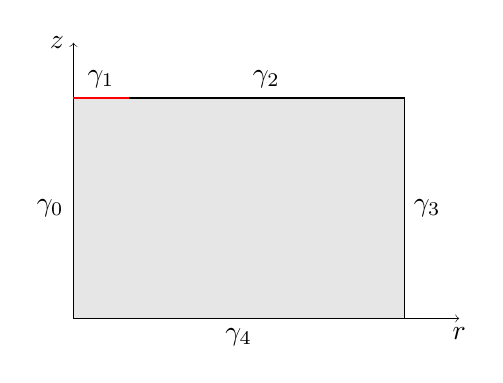
\begin{tikzpicture}[scale=0.7]
	% axes
	\draw [->, very thin] (0, 0) -- (7, 0) node[below] {$r$};
	\draw [->, very thin] (0, 0) -- (0, 5) node[left] {$z$};

	% rectangle
	\draw [fill=gray, fill opacity=0.2] (0, 0) -- (6, 0) -- (6, 4) -- (0, 4) -- cycle;

	% labels
	\node[left] at (0, 2) {$\gamma_0$};
	\node[above] at (0.5, 4) {$\gamma_1$};
	\node[above] at (3.5, 4) {$\gamma_2$};
	\node[right] at (6, 2) {$\gamma_3$};
	\node[below] at (3, 0) {$\gamma_4$};

	\draw [red] (0, 4) -- (1, 4);
\end{tikzpicture}

		\caption{Cylinder $\Omega$, its boundaries and the radial section.}
	\end{figure}
\end{frame}


\begin{frame}{Boundary conditions}
We consider the energy transferred to the body via the laser beam as a heat flux through the part of the boundary $\Gamma_1$:
\begin{equation}
	\kappa(\theta(x,t)) \frac{\partial \theta(x,t)}{\partial \vec{n}} = - \eta \cdot \text{pd}_{\max} \cdot u(t).
\end{equation}
Here $\text{pd}_{\max}$ is the power density of the laser beam, $\eta$ is the absorption coefficient of the material, and $u(t)$ is the control function bounded by $[0,1]$.

The cooling of the body is described as a heat flux through the whole boundary, except possibly $\Gamma_3$ (the choice of a boundary condition at the lateral surface $\Gamma_3$ makes no essential difference if the radius of $\Omega$ is chosen big enough).
We distinguish a convective and a radiative cooling heat fluxes modelled as
\begin{equation}
	\kappa(\theta(x,t)) \frac{\partial \theta(x,t)}{\partial \vec{n}} = h \cdot (\theta(x,t) - \theta_\text{amb})
\end{equation}
and
\begin{equation}
	\kappa(\theta(x,t)) \frac{\partial \theta(x,t)}{\partial \vec{n}} = k \cdot (\theta(x,t)^4 - \theta^4_\text{amb})
\end{equation}
respectively.
Here $k$ and $h$, are the radiative and the convective cooling coefficients respectively, and $\theta_\text{amb}$ is the ambient temperature.
\end{frame}


\begin{frame}{Model equations}
The temperature distribution in $\Omega$ is described by the quasi-linear heat equation
\begin{equation} \label{eq:heat_eq}
	s(\theta(x,t)) \frac{\partial \theta(x,t)}{\partial t} = \div (\kappa(\theta(x,t)) \grad\theta(x,t))
\end{equation}
where $s(\theta(x,t)) \coloneqq c(\theta(x,t)) \rho(\theta(x,t))$.

While the first spot of the welding seam is considered, the initial temperature $\theta(x,0)$ inside $\Omega$ is assumed to be constant and equal to the ambience temperature $\theta_\text{amb}$.

The boundary conditions are
{\small
\begin{equation}
	\kappa(\theta(x,t)) \frac{\partial \theta(x,t)}{\partial \vec{n}} = \left\{
		\hspace{-0.5em}
		\begin{array}{ll}
			k (\theta(x,t)^4 - \theta_\text{amb}^4) + h (\theta(x,t) - \theta_\text{amb}) - \eta\, \text{pd}_{\max} u(t), & \text{on}\ \Gamma_1, \\
			k (\theta(x,t)^4 - \theta_\text{amb}^4) + h (\theta(x,t) - \theta_\text{amb}), & \text{on}\ \Gamma_2 \cup \Gamma_4, \\
			0, & \text{on}\ \Gamma_3.%
		\end{array} \right.
\end{equation}
}
\end{frame}


\begin{frame}{Motivation for optimization} 
The objective functional is constructed a sum of independent penalty terms, each term corresponding to a certain application driven requirement.
We try to avoid state constraints as far as possible.

\begin{block}{As imposed by the application, the desired optimal control must:}
	\begin{enumerate}[label=(\arabic*)]
		\item provide sufficient welding penetration;
		\item ensure complete solidification withing a preselected time interval;
		\item avoid hot cracking during the solidification stage;
		\item minimize the total energy consumed by the laser.
	\end{enumerate}
\end{block}

Let us now derive the penalty terms corresponding to each of these requirements.
\end{frame}


\begin{frame}{Objective functional}
	Welding penetration:
	\begin{equation}
		J_{\text{penetration}} = \frac{\beta_\text{penetration}}{2} \left( \| \theta(x_{\text{target}},\cdot) \|_{L^{\infty}[0,T]} - \theta_{\text{threshold}} \right)^2,
	\end{equation}

	Solidification completeness:
	\begin{equation}
		J_{\text{completeness}} =
		\frac{\beta_\text{completeness}}{2} \int_{\Omega} \max\{ \theta(x, T) - \text{solidus},\ 0 \}^2\, dx.
	\end{equation}

	Minimizing energy consumption:
	\begin{equation}
		J_\text{control} =
		\frac{\beta_\text{control}}{2} \|u(t)\|^2_{L^2[0,T]}.
	\end{equation}
\end{frame}


\begin{frame}{Objective functional: avoiding hot cracking}
Let $I(t)$ be a moving over time isothermal surface in $\Omega$. For a moving point $x(t) \in I(t)$ one can get
\begin{equation} \label{eq:dxt}
	\frac{d}{dt} \theta(x(t),t) = \grad \theta(x(t),t) \cdot x_t(t) + \theta_t(x(t),t) = 0.
\end{equation}
The derivative $x_t(t)$ can be decomposed as
\begin{equation} \label{eq:xt_alpha_beta}
	x_t(t) = \alpha(x(t),t) \cdot \grad \theta(x(t),t) + \beta(x(t),t) \grad \theta(x(t),t)^{\top}
\end{equation}
where $\alpha(x(t),t)$ and $\beta(x(t),t)$ are scalar functions. From these equations we get
\begin{equation}
	\alpha(x(t),t) = \frac{\theta_t(x(t),t)}{\|\grad \theta(x(t),t)\|^2}.
\end{equation}
	\vspace{-2em}
	\begin{figure}
		\centering
		\includegraphics[width=0.75\linewidth]{plots/static/velocity.pdf}\\
		\vspace{-2em}
		\caption{Velocity of an isothermal surface.}
	\end{figure}
\end{frame}


\begin{frame}{Objective functional: avoiding hot cracking}
	Therefore, we define the velocity of an isothermal surface as
	\begin{equation}
		v(x,t) \coloneqq \frac{\theta_t(x,t)}{\|\grad \theta(x,t)\|}.
	\end{equation}

	We are only interested in restricting negative values within the solidus-liquidus temperature corridor:
	\begin{equation}
		J_{\text{velocity}} = \frac{\beta_\text{velocity}}{2} =
		\int_{\Omega \times [0,T]} \max \{ v_{\max} - v(x,t),\ 0 \}^2 \cdot \chi(\theta(x,t))\, dx\,dt
	\end{equation}
	\begin{equation}
		\chi(\theta) \coloneqq \left\{
			\begin{array}{ll}
				1, & \text{if}\ \text{solidus} \le \theta \le \text{liquidus}, \\
				0, & \text{otherwise}.
			\end{array} \right.
	\end{equation}
\end{frame}


\begin{frame}{Numerical results: linear rampdown}
	Conventional laser pulse welding strategies use a rectangular laser pulse shape.
	Unfortunately, this often leads to hot-cracking when applied to aluminum alloys.

	A so-called linear rampdown pulse shape has shown its potential to maintain a crack-free welding of aluminum alloys.
	However, ramp-down pulses are not likely to be optimal with respect to any of the criteria listed before.
	\begin{table}
		\centering
		\input{tables/rampdown}
		\caption{Numerical report on simulations with the conventional and the linear rampdown pulse shapes, and based on them optimized * pulse shapes.}
		\label{tab:rampdown}
	\end{table}
\end{frame}


\begin{frame}{Numerical results: linear rampdown}
	\begin{figure} 
		\centering
		\includegraphics{plots/optimized/rampdown.pdf}
		\caption{Solutions to the optimal control problem with conventional (left) and linear rampdown (right) pulse shapes taken as initial guesses.}
		\label{fig:rampdown}
	\end{figure}
\end{frame}


\begin{frame}{Numerical results: optimizations from zero initial guess}
	In the search for obtain better pulse shapes, we now begin with the trivial initial guess $u_\text{initial} \equiv 0$ with no power radiated by the laser.

	With this initial guess, the target temperature is clearly not reached and the term $J_\text{penetration}$ drives the pulse shape away from its initial value.
	
	\begin{table}
		\centering
		\input{tables/zeroguess}
		\caption{Numerical report on the series of optimizations with zero initial guess.}
		\label{tab:zeroguess}
	\end{table}
\end{frame}


\begin{frame}
	\vspace{-0.75em}
	\begin{figure}
		\centering
		\includegraphics{plots/optimized/zeroguess.pdf}
		\vspace{-1.0em}
		\caption{Solutions to the optimal control problem with zero initial guess with the variable maximal laser power (vertical) and maximal welding time (horizontal) parameters.}
		\label{fig:zeroguess}
	\end{figure}
\end{frame}


\begin{frame}{The end}
	\begin{center}
		\texttt{{\textbackslash}end\{talk\}}\\[1em]
		\vfill
		\begin{tabular}{rl}
			\textbf{this talk} & \url{https://github.com/optipulsproject/talk-bayreuth} \\
			\textbf{preprint} & \url{https://github.com/optipulsproject/paper-onespot} \\
			\textbf{numerical model} & \url{https://github.com/optipulsproject/optipuls} \\
			\textbf{makeresearch tutorial} & \url{https://github.com/dstrelnikov/makeresearch}
		\end{tabular}
	\end{center}
\end{frame}
\end{document}
